\documentclass[entwurf]{uebblatt}

\newcommand{\http}{http:/\kern-.2em/\kern-0.03em}

\begin{document}

\maketitle{6}{}

\begin{aufgabe}{2+m+1}{Ein konkretes Beispiel für eine Primärzerlegung}
Sei~$K$ ein Körper. Seien die Ideale~$\ppp_1 = (X,Y)$, $\ppp_2 = (X,Z)$
und~$\mmm = (X,Y,Z)$ von~$K[X,Y,Z]$ gegeben. Sei~$\aaa = \ppp_1 \ppp_2$.
\begin{enumerate}
\item Zeige, dass~$\aaa = \ppp_1 \cap \ppp_2 \cap \mmm^2$ eine minimale
Primärzerlegung von~$\aaa$ ist.
\item Welche Primideale von~$K[X,Y,Z]$ sind zu~$\aaa$
isolierte Primideale, welche eingebettete?
\item Schreibe die assoziierten Primideale in der Form~$\sqrt{(\aaa:f)}$ für
geeignete~$f \in K[X,Y,Z]$.
\end{enumerate}
\end{aufgabe}

\begin{aufgabe}{2+m+2}{Erweiterungen primärer Ideale in Polynomringen}
Sei~$A$ ein Ring.
\begin{enumerate}
\item Sei~$\qqq$ ein~$\ppp$-primäres Ideal
in~$A$. Zeige, dass~$\qqq[X]$ ein~$\ppp[X]$-primäres Ideal in~$A[X]$ ist.
\item Sei~$\aaa = \qqq_1 \cap \cdots \cap \qqq_n$ eine minimale Primärzerlegung
in~$A$. Zeige, dass~$\aaa[X] = \qqq_1[X] \cap \cdots \cap \qqq_n[X]$ eine
minimale Primärzerlegung in~$A[X]$ ist.
\item Zeige: Ist~$\ppp$ ein zu einem zerlegbaren Ideal~$\aaa$ isoliertes Primideal, so
ist~$\ppp[X]$ ein zu~$\aaa[X]$ isoliertes Primideal.
\end{enumerate}
\end{aufgabe}

\begin{aufgabe}{2+2}{Ein Kriterium für Assoziiertheit}
Sei~$\aaa$ ein Ideal eines Rings~$A$.
Sei~$\ppp$ ein Ideal, das unter allen Idealen der Form~$(\aaa:x)$ mit~$x
\in A$ und~$x \not\in \aaa$ maximal ist.
\begin{enumerate}
\item Zeige, dass~$\ppp$ ein Primideal ist.
\item Sei~$\aaa$ zerlegbar. Zeige, dass~$\ppp$ ein zu~$\aaa$ assoziiertes
Primideal ist.
\end{enumerate}
\end{aufgabe}

\begin{aufgabe}{0+2+2+m}{Erste Schritte mit ganzen Erweiterungen}
\begin{enumerate}
\item Seien~$x$ und~$y$ Elemente eines Rings, die vermöge der
Gleichungen~$x^2-3x+1=0$ und~$y^2+5y-2=0$ über~$\ZZ$ ganz sind. Finde eine
Ganzheitsgleichung für~$x+y$.
\item Sei~$A \subseteq B$ eine ganze Ringerweiterung. Sei~$x$ ein Element
von~$A$, das in~$B$ invertierbar ist. Zeige, dass~$x$ schon in~$A$ invertierbar ist.
\item Sei~$A \subseteq B$ eine Ringerweiterung. Sei~$C$ der ganze Abschluss
von~$A$ in~$B$. Seien~$f,g \in B[X]$ normierte Polynome mit~$fg \in C[X]$.
Zeige, dass~$f \in C[X]$ und~$g \in C[X]$.
\item Sei~$G$ eine endliche Gruppe von Automorphismen eines Rings~$A$. Zeige,
dass~$A$ über dem Unterring~$A^G \defeq \{ x \in A \,|\, \text{$g(x)=x$ für
alle $g \in G$} \}$ ganz ist.
\end{enumerate}
\end{aufgabe}

\centering
\begin{center}
  \rotatebox{90}{\tiny\sffamily \http www.smbc-comics.com/?id=3565}
  \href{http://www.smbc-comics.com/?id=3565}{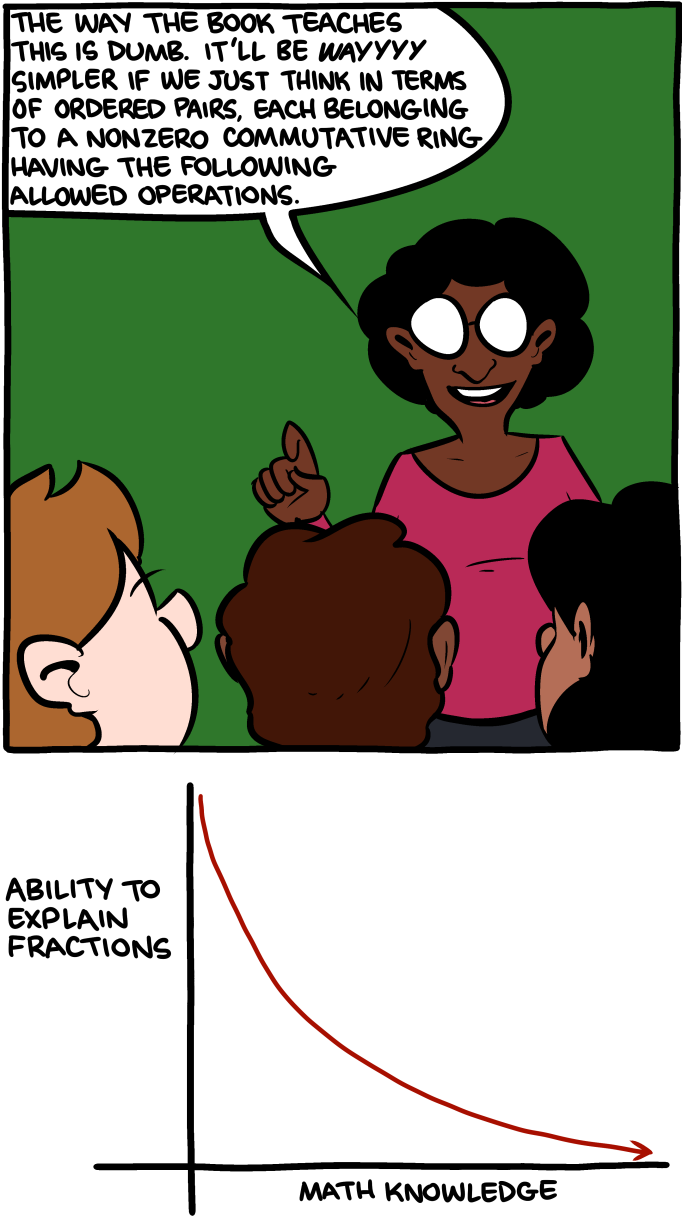
\includegraphics[angle=90,height=4.5cm]{images/smbc-fractions}}
\end{center}

\end{document}
